\appendix
\section{Projection Details}\label{Sec:Projection}
To enforce the divergence constraint in {\bf Step 3, 7}, and {\bf 11}, we use a projection method analgous to the methods originally developed for incompressible flow \citep{almgren1998conservative,bell1989second}.
The basic idea is to decompose the velocity field into a divergence-free component and a curl-free (gradient of a scalar field) component by solving a variable-coefficient Poisson equation for the scalar field.
The details for the MAC projection in {\bf Step 3} and {\bf Step 7} are given in Appendix B of Paper III.  The details of the nodal projection in {\bf Step 11} are given in Section 3.2 of Paper III.
We note that in the nodal projection, the gradient of the scalar field is used to update the perturbational pressure, $\pi$.

Based on our past experience in the MAESTRO project, we have found it useful to split the velocity dynamics into a perturbational and base state velocity,
\begin{equation}
\Ub = \Ubt(\xb,t) + w_0(r,t)\eb_r,
\end{equation}
solve for each term separately, and immediately combine them to find a full velocity that satisfies the constraint.  We take that approach here, primarily because it allows us to enforce a boundary condition on $w_0$ at the edge of the star (i.e., the cutoff density location where we hold density constant).  Namely, to enforce that $r^2 w_0$ remain constant is difficult to do when solving for the full velocity.  So in practice, we solve the constraint over the lateral average,
\begin{equation}
\nabla\cdot\left(\beta_0\Ubt\right) = \beta_0(S-\overline{S})
\end{equation}
and sepratately solve for $w_0$ using 
\begin{equation}
\nabla\cdot(\beta_0w_0\eb_r) = \beta_0\left(\overline{S} - \frac{1}{\gammaonebar p_0}\frac{\partial p_0}{\partial t}\right).
\end{equation}
To solve for $\Ubt$ we use a projection method, which involves the solution of a variable-coefficient Poisson solver to extract the curl-free component of the unprojected velocity.
Note that MAESTRO contains alternate low Mach number formulations that conserve total energy in stratified systems, with minimal changes to the code (see Appendix A of \cite{subChandra_II} for details).
To find $w_0$ we integrate in 1D using the procedure in Appendix B of Paper V.
Note that in this approach, we estimated the time-derivative of the pressure in part by examining how laterally averaged $\rho'=\rho-\rho_0$ changed over time (quantified by $\eta_\rho = \overline{\rho'\Ub\cdot\eb_r}$).  After evolving the species, we compute this term in the same way as reported in Paper V for use in computing $w_0$.
\MarginPar{mention changes in $w_0$ computation for irregular base state. Add graphic of temperature falling due to incorrect splitting?}

%%%%%%%%%%%%%%%%%%%%%%%%%%%%%
\begin{figure}[htb]
\begin{center}
\begin{tabular}{l r}
\multirow{4}{3.5in}[34.5mm]{ 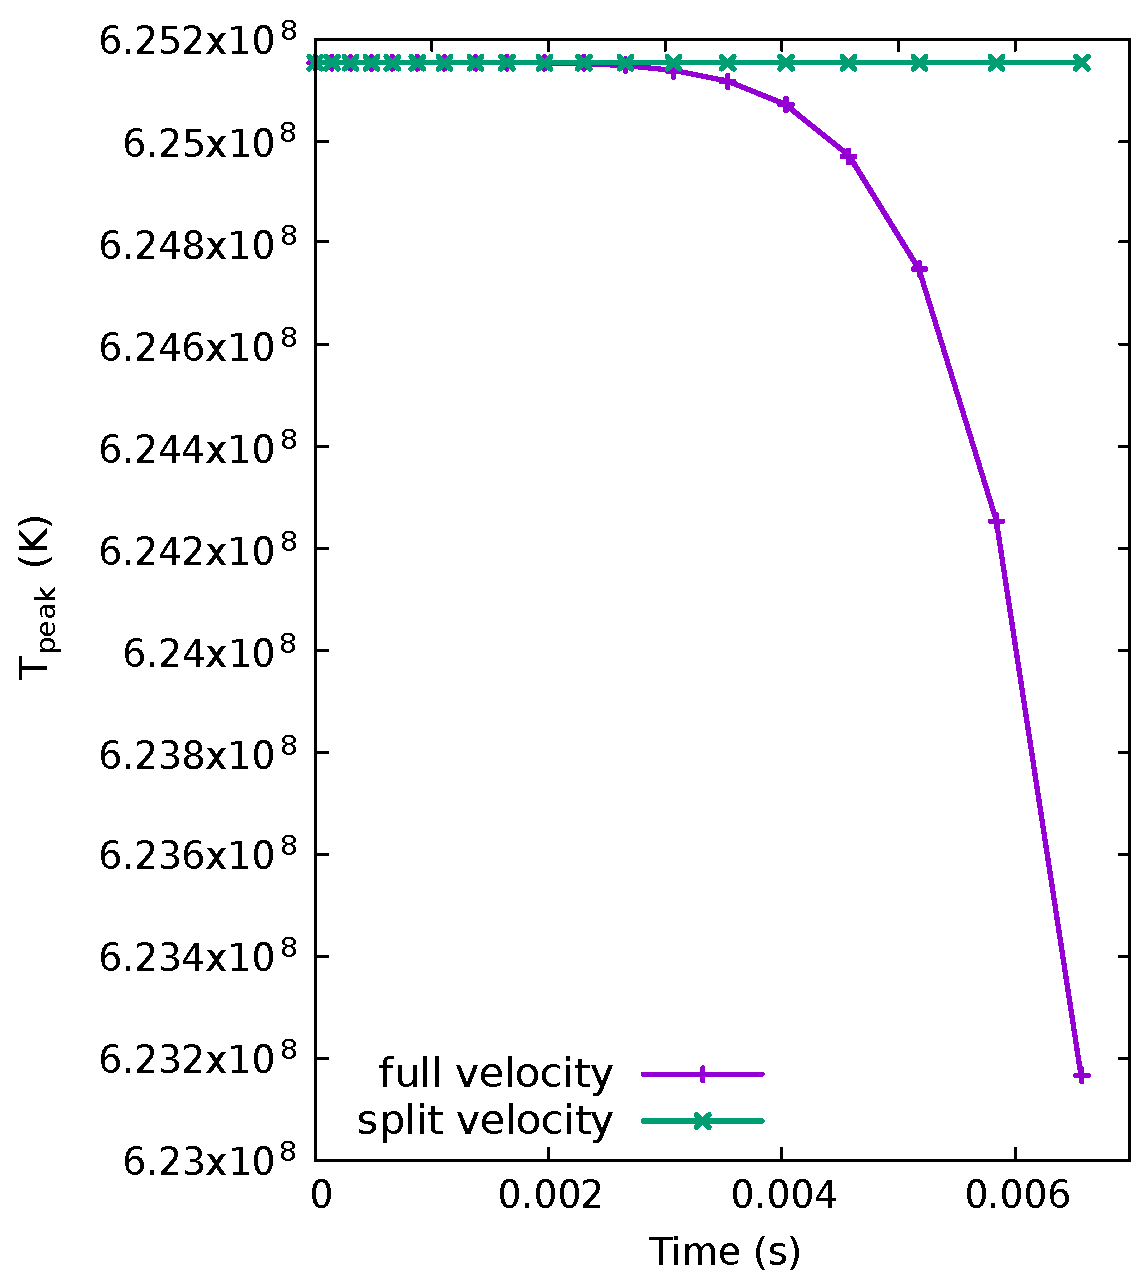
\includegraphics[width=3.0in]{./figs/wdconvect_256_splitU} } & \multicolumn{1}{c}{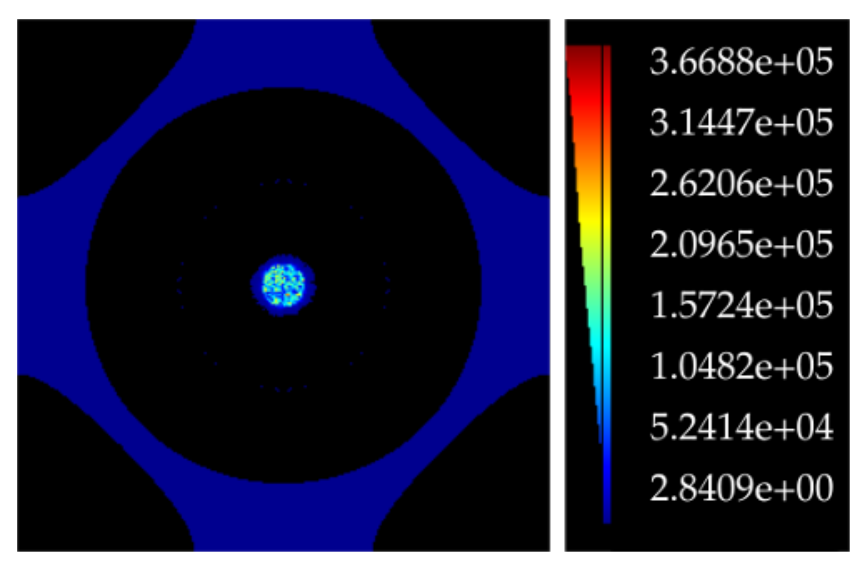
\includegraphics[width=2.35in]{./figs/magvel_full_XY}} \\
& \multicolumn{1}{c}{\begin{footnotesize} (a) $|\mathbf{U}|$, solved using $\mathbf{U}$ \end{footnotesize}} \\[1.em]
& \multicolumn{1}{c}{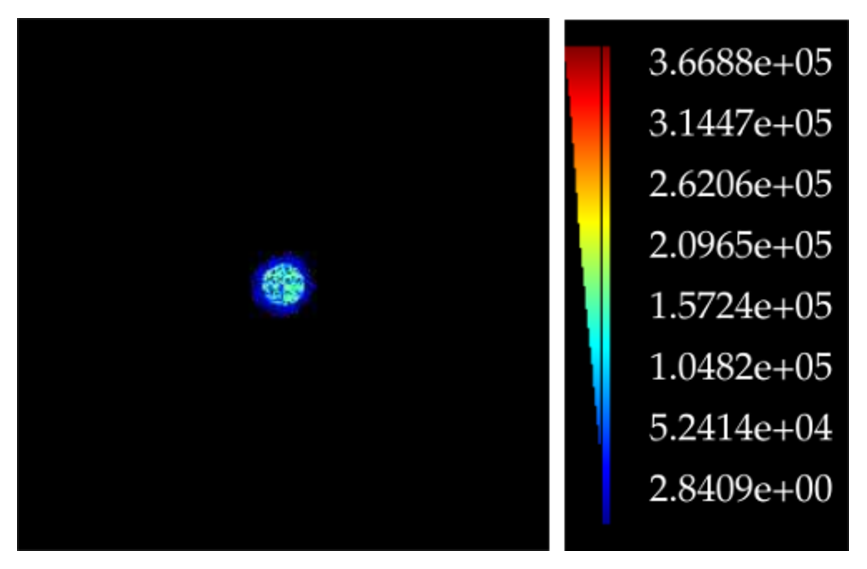
\includegraphics[width=2.35in]{./figs/magvel_split_XY}} \\ 
& \multicolumn{1}{c}{\begin{footnotesize} (b) $|\mathbf{U}|$, solved using $w_0 + \tilde{\mathbf{U}}$ \end{footnotesize}} \\
\end{tabular}
\caption{\label{fig:wdconvect_splitU} (Left) Peak temperature, $T_{\text{peak}}$ in a white dwarf at resolution of $256^3$ 
         during initial transition. (Right) Velocity magnitude solved using the full velocity $\mathbf{U}$ in projection step 
         results in large values outside the density cutoff region that is not seen with using the split velocities.}
\end{center}
\end{figure}
%%%%%%%%%%%%%%%%%%%%%%%%%%%%%

\section{Old Notes (not for inclusion in paper)}

\subsection{Exact Base State Notes}

\subsubsection{Potential Problems}
\begin{enumerate}
\item How do we define \verb|r_edge_loc| for irregularly-spaced base states whose cell-centered values are defined at $r_m=\Delta x\sqrt{\frac{3}{4} + 2m}$?
\item We would stil need to approximate the values at edges when advecting the base states (i.e. $\rho_0^{\nph,\pred}$). This may affect the nice properties we would get with exact cell-centered base state values.
\item Excessive memory storage may be required (\verb|nr_irreg >> nr_fine|).
\end{enumerate}

\subsubsection{A Possible Solution}
We could choose to no longer advect the base states for both predictor and corrector steps. This would solve the problems with computing state values at cell edges. Instead, we propose to only update the base states $\rho_0$ and $p_0$ by computing the average of the full state values after advecting the full states. This would result in the following changes in the algorithm from Paper V:
%
\begin{enumerate}
\item Steps 4 and 8 will be greatly simplified, leading to a more efficient algorithm.
\item \sout{There is no longer a need for $w_0$, so we can use the full velocity $\Ub$ instead of $\Ubt$. As a consequence, $\eta$ does not need to be computed. This has the added advantage of saving some memory storage by removing many of the terms needed when we decided to split terms into its base state and perturbation state in our previous implementation.} We split the velocity for the projection to handle the cutoff.
\item By placing the base states exactly at cell-centers, we eliminate interpolation errors and simplify the existing code.
\end{enumerate}
%

\subsection{$\eta_\rho$ Notes}
After {\bf Step 8D}, we define a radial cell-centered $\etarho^{\nph}$.

\begin{description}
\item For planar geometry, $\etarho = \overline{\rho'(\Ub\cdot\eb_r)}$,
\begin{equation}
 \etarho^{\nph} =  {\rm {\bf Average}} \sum_k \left[ \left(\uadvtwo \cdot \eb_r \right) (\rho X_k)^{\nph,\pred} \right]
\end{equation}
\item For spherical geometry, first construct 
$\etarho^{{\rm cart},\nph} = [\rho'(\Ub\cdot\eb_r)]^{\nph}$ on Cartesian cell centers using:
\begin{equation}
\etarho^{{\rm cart},\nph} = \left[\left(\frac{\rho^{(1)}+\rho^{(2)}}{2}\right)-\left(\frac{\rho_0^n+\rho_0^{n+1}}{2}\right)\right] \cdot \left( \uadvtwo \cdot \eb_r \right).
\end{equation}
Then,
\begin{equation}
\etarho^{\nph,\star} = {\rm {\bf Average}}\left(\etarho^{{\rm cart},\nph}\right).
\end{equation}
\end{description}

\subsection{Computing $w_0$ For Spherical Problems}
Recall that we want to solve
\begin{equation}
\frac{1}{r^2}\frac{\partial}{\partial r}(r^2 w_0) = \Sbar - \frac{1}{\gammaonebar p_0}\left(\frac{\partial p_0}{\partial t} + w_0\frac{\partial p_0}{\partial r}\right)
\end{equation}
First, note that $\partial p_0/\partial r = -\rho_0 g$.
The key observation here is that we can compute $\partial p_0/\partial t$ directly instead of making complicated substitutions involving $\eta_\rho$ to eliminate it.
Let's discretize this as follows:
\begin{equation}
\frac{1}{r_j^2}\left[\frac{\left(r^2 w_0\right)_{j+\myhalf} - \left(r^2 w_0\right)_{j-\myhalf}}{\Delta r}\right] = 
\Sbar_j - \frac{1}{\left(\gammaonebar p_0\right)_j}\left[\left(\frac{\partial p_0}{\partial t}\right)_j - \left(\frac{w_{0,j-\myhalf}+w_{0,j+\myhalf}}{2}\right)(\rho_0 g)_j\right]
\end{equation}
Rearranging this to solve for $w_{0,j+\myhalf}$ gives us an explicit update:
\begin{equation}
\left[\frac{r_{j+\myhalf}^2}{r_j^2\Delta r} - \frac{(\rho_0 g)_j}{2\left(\gammaonebar p_0\right)_j}\right] w_{0,j+\myhalf} =
\left[\frac{r_{j-\myhalf}^2}{r_j^2\Delta r} + \frac{(\rho_0 g)_j}{2\left(\gammaonebar p_0\right)_j}\right] w_{0,j-\myhalf}
+ \Sbar_j - \frac{1}{\left(\gammaonebar p_0\right)_j}\left(\frac{\partial p_0}{\partial t}\right)_j
\end{equation}
As before, once $\rho_0$ falls below $\rho_{\rm cutoff}$, we hold $r^2 w_0$ constant.\\ \\
The interface to the routine in the algorithm description is
{\bf Make $\mathbf{w_0}$}$[\rho_0,p_0,\partial p_0/\partial t,\gammaonebar,\Sbar] \rightarrow [w_0]$

\subsection{TODO List}

TODO list:
\begin{itemize}
\item Weak scaling tests of original algorithm, comparing MAESTRO to MAESTROeX.  Use cori knl, 4 MPI per node, 16 threads per MPI
\item Run at effective $512^3$ resolution (maybe to ignition?... need to see how max T trends go) (1) classic MAESTRO, (2) MAESTROeX with original algorithm, (3) MAESTROeX with new temporal integrator, (4) MAESTROeX with new temporal integrator and irregular dr, (5) MAESTROeX with original algorithm and 3-levels of AMR, (6) MAESTROeX with new temporal integrator and 3 levels of AMR.
\item (perhaps) a demonstration of what goes wrong when you don't split the velocity dynamics in the projection
\end{itemize}

